
\documentclass[article, 10 pt, conference]{ieeeconf} 

\overrideIEEEmargins

\usepackage{graphicx}
\usepackage{hyperref}
\usepackage[section]{placeins} 

\pagestyle{plain}


% The following packages can be found on http:\\www.ctan.org
%\usepackage{epsfig} % for postscript graphics files
%\usepackage{mathptmx} % assumes new font selection scheme installed
%\usepackage{mathptmx} % assumes new font selection scheme installed
%\usepackage{amsmath} % assumes amsmath package installed
%\usepackage{amssymb}  % assumes amsmath package installed

\title{\LARGE \bf
New York City Uber Pickup Analysis and Prediction
}

\author{Chuan Chen, Yafu Ruan, Shuwen Shen, Yihang Zhang}


\begin{document}



\maketitle


\section{INTRODUCTION}

The demand for ride-sharing services in NYC can vary in different areas, time periods, or under different weather conditions. Based on the Kaggle dataset of NYC Uber Pickups for 6 months starting from January 2015, we aimed to analyze and predict the demand (measured and represented by the number of pickups) and to analyze the relationships between the number of pickups and variables including weather, location, and several time factors. We try to produce results that could provide insights to help ride-sharing companies like Uber improve the user experience through optimizations in planning.

\section{Data Overview}

\subsection{Dataset Description}

Our dataset ?NYC Uber Pickups with Weather and Holidays? comes from Kaggle [1]. The dataset consists of the hourly data collected from 01/01/2015 to 30/06/2015. 

Overall, the dataset contains 29,101 instances, each of which has the following 13 variables:

\begin{table}[h]
\caption{data overview}
\label{tab:data}
\begin{center}
\begin{tabular}{|c|c|}
\hline
feature & definition\\
\hline
\hline
pickup\_dt & Time period of the observations\\
\hline 
borough & NYC's borough\\
\hline pickups& Number of pickups for the period\\
\hline spd& Wind speed in miles/hour\\
\hline vsb& Visibility in Miles to nearest tenth\\
\hline temp& temperature in Fahrenheit\\
\hline dewp& Dew point in Fahrenheit\\
\hline slp& Sea level pressure\\
\hline pcp01& 1-hour liquid precipitation\\
\hline pcp06& 6-hour liquid precipitation\\
\hline pcp24& 24-hour liquid precipitation\\
\hline sd& Snow depth in inches\\
\hline hday& Being a holiday (Y) or not (N)\\
\hline
\end{tabular}
\end{center}
\end{table}


\begin{figure}[!h]
    \includegraphics[width=0.47\textwidth]{bar1:2.png}
    \includegraphics[width=0.47\textwidth]{bar2:2.png}
    \caption{Bar plot of the relationship between 4 features to pickup amount }
\end{figure}


\subsection{Exploratory Data Analysis}
We applied several data visualization techniques trying to discover how different features would affect Uber ridership.

From the bar plot in terms of the number of pickups and borough, we could see that Manhattan, not surprisingly, accounts for the largest number of Uber pickups of any borough, and EWR produces the smallest. Weather events, for example, the snowfall, would definitely have significant impact on daily Uber ridership. According to the bar plot of snow depth variable, it appears that when snow depth is greater than 6 inches, the amount of Uber pickups would significantly increase. 

We also constructed a heat map to show the pattern and magnitude of the number NYC Uber pickups in terms of month and hour.
\begin{figure}[!htb]
    \includegraphics[width=0.45\textwidth]{heatmap.png}
    \caption{Heatmap generated by Python Seaborn  reflecting Uber pickups values during a day over 6 months.}
\end{figure}
on every night after 5pm from January to June, among all 6 months, Uber provides more trips than any other time periods and reaches its peak during the whole day. This is probably because people are more likely to feel tired after a long day of work, so that they tend to rely on Uber pickup system to rush home or enjoy dinner time with friends. Also, we found that the Uber ridership in February and June is relatively high compared to other months. This could be explained by the inclement weather temperature during February and June.


\section{Data Preprocessing}

\subsection{Missing Values} 

There is one type of missing values (?NaN?) in one of the columns (?borough?) in our dataset. We checked that 3043 out of 29101 (total) records had ?NaN?. Since this represents a small proportion of the total data available, we decided to drop the records containing missing values. 

\subsection{String Values} 

There are two columns with string values in our dataset - ?hday? and ?borough?. We transformed both to numerical columns. Specifically, ?Hday? has values ?Y? (if it is a holiday) and ?N? (if it is not a holiday). We transformed the values into 1 (for ?Y?) and 0 (for ?N?)

\subsection{Dummy Variables}

For regression models, we use one-hot encoding to convert borough feature into six dummy variables with names "Bronx", ?Brooklyn?, ?EWR?, ?Manhattan?, ?Queens?, and ?Staten Island?. A record has a value of ?1? if it belongs to the borough that the dummy variable represents and ?0? if not.

\subsection{Date Features}

The original date feature is not in pandas date time format. Therefore, we converted it into different features based on the demands of different models, which will be specified in the Modeling section.

\subsection{Feature Normalization}

According to that most of the features in our dataset are having greatly different scale, we applied normalization on numerical features so as to fit the model better.



\section{Modeling}

\subsection{Linear Regression Model}

As our baseline model, we expected to extract the linear relationship between features and target variable so as to understand how pickup amount is influenced by those features. 

To process the date feature, we converted it into three categorical features, day, month and range. Day refers to the exact date within month, from 1 to 31. Month refers to the exact month of the record, from 1 to 6 since the dataset only cover January to June. And range refers to 8 three-hour ranges(e.g. 1 means 1 am to 3 am, 2 means 4am to 6 am). 

After we splited the dataset, we fitted the model and checked the multicollinearity. The R-squared was 0.701 and the RMSE was 0.08346, which was not bad. While looking at the detailed summary, we noticed that several features were statistically insignificant and some pairs of features had serious multicollinearity problem, such as dew point and temperature. Therefore, after feature selection, the model got improved a little and all kept features were now statistically significant. However, by looking at coefficients, we found it was difficult to explain the influence of date features on the target variable. The reason might be that the model would take date features as numerical features instead of categorical features since they were highly ordinal.

In this case, we simply excluded the date features for linear regression to see how the rest features affect the target variables without considering time. The R square went down to 0.660 since we decrease the feature amount but the F Statistics went up from 2190 to 3660, which indicates a better fit and model explanation. 

\begin{figure}[!htb]
     \includegraphics[width=0.5\textwidth]{LR_summary.png}
    \caption{Coefficients of Linear Regression }
\end{figure}

The current model seems better, with a higher F statistics and lower RMSE. It is acceptable for R Square experiencing a decrease because less features are included. Almost all of the features are statistically meaningful except Queens but we need to keep it. By looking at the coefficients, we can see features positively influencing the pickup amounts are: windspeed, temperature, Brooklyn and Manhattan, meaning that with higher windspeed, temperature, or when place is in Brooklyn and Manhattan, we expect higher amount of pickups. Vice Versa with the rest features.


\subsection{Elastic Net}

In the linear regression model, we manually filtered the features when dealing with multicollinearity. Therefore, we wanted to applied Elastic Net Model by adding regularization term to automatically shrink and penalize features. To determine the parameters, we applied MPI to accelerate the grid searching process. As the result, when alpha is 0.0011 and l1 ratio is 0.1, we get the best model with 0.7246 as R2 and 0.0836 as RMSE.

\begin{figure}[!htb]
    \includegraphics[width=0.5\textwidth]{EN_Summary.png}
    \caption{Coefficients of Elastic Net Model }
\end{figure}

According to the output, we got how the features in this model linearly influence the target feature. Some of the features' coefficients have been shrinked to 0, indicating they are filtered out because of multicollinearity. Most of them are exactly the features have been dropped in Linear Regression Model.


\subsection{ARIMA}

Since our Uber pickups data is collected hourly in sequential order, it is a time series in nature. Thus, it would make sense to try analyzing the data using time series models, such as the ARIMA model. The downside of evaluating the dataset using the ARIMA model is that all features beside time are discarded, and their collection efforts are wasted. However, the upside is that it can capture the strong time dependency apparent in the data, something that ordinary machine learning models can not do. Since the same time point repeats 6 times in our dataset, one for each borough, we are faced with 2 options to prepare our dataset for time series analysis. We can either take the average pickup numbers across all 6 boroughs for each time point, or we can split the dataset into 6 sub-dataset and perform time series analysis on each borough-specific data frames. Since each borough differs significantly from each other, averaging them all together would cause us to lose insight into the area-specific effects on the pickup numbers. During deployment, allowing Uber drivers and consumers to see the prediction for the specific borough they are located in will certainly be more helpful then providing them with the average pickup numbers across the entire City. Thus, we have decided to split our data into 6 borough-specific data sets. Then, all features beside time are discarded, and the data was normalized. From the decomposition for the Bronx dataset, as shown in figure \ref{fig:bronx_decomp}, we can clearly observe a daily periodicity pattern, and the same seasonality is apparent in all other data sets. 
\begin{figure}[!htb]
    \includegraphics[width=0.45\textwidth]{bronx_decomp.png}
    \caption{times-series decomposition for the Bronx dataset}
    \label{fig:bronx_decomp}
\end{figure}
The ARIMA model was fitted on each of the 6 data sets, and a total of 64 different parameters was tested on each fit, setting the periodicity to be 24. The best parameter for each fit was selected based on the lowest AIC score, which is an indicator that balances goodness of fit and model complexity. Afterwards, the models were refitted on each of the 6 data sets using their corresponding best parameters. The result of each fit is shown in appendix \ref{app:model_results}. Figure \ref{fig:bronx_res} shows that the residual after the ARIMA fit is near normally distributed, which suggest that they are random noise, and we have extracted most of the pattern from our data.
\begin{figure}[!htb]
    \includegraphics[width=0.45\textwidth]{bronx_res.png}
    \caption{residuals for the Bronx model}
    \label{fig:bronx_res}
\end{figure}
The residuals for the rest of the models are shown in appendix \ref{app:model_residuals}. All model residuals are nearly normally distributed. An in-sample prediction was performed for all data sets for a 15-day period. Results are shown in appendix \ref{app:model_pred}. The average prediction RMSE is 0.0690. An out of sample forecast was conducted for a 36-day period and compared with the validation set. Results are shown in appendix \ref{app:model_fore}. The final average forecast RMSE is 0.1645.

\subsection{Neural Network}

We also uses Neural Network as to deal with the nonlinear relationship between the features and target variables. Here mean square error was used as the objective function.

Here we also introduce MPI to speed up the gridsearching for hyperparameters. For this problem we find out that a deep network may not be a good choice, so we design a simple only two hidden layers. Relu is chosen as the activation function and the slover is set to be adam after parameter tuning.

The network converges within 50 epoch and and MSE on training set reaches 0.0024 as shown in figure 5. We also introduce the early stopping technique to avoid overfitting.
\begin{figure}[!htb]
    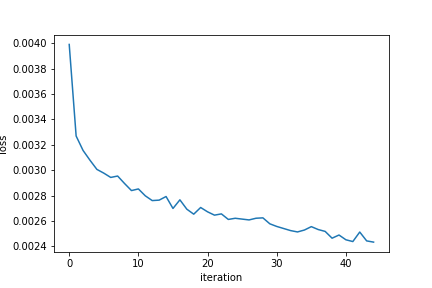
\includegraphics[width=0.45\textwidth]{network_loss.png}
    \caption{Training loss on neural network}
\end{figure}

Finally the RMSE on the validation set is 0.0703, which is slightly better than linear models. However this model is hard to explain and it's difficult to find the relationship between features and variables.


\section{Performance Improving}
\subsection{line\_profiler}
The line\_profiler shows how much time is spent one each function. It helps us understand which line actually causes the program slow and it may be obvious enough. In our project, we first use line\_profiler to locate the part that need to be optimized and then apply several techniques.
\subsection{Itertools}
The itertools provides a number of iterators that is fast and efficient compared with operation on list. The reason is that itertools do not produce the data until it is needed. Since it reduce the swag between data, it speed up the program in large dataset. We use itertools in gridsearching part to find all combinations of hyperparameters. It shows that using list operations will take more time. While setting up the hyperparameter search grids for the ARIMA model, a for-loop took 0.0052s, while an itertools method only took 0.0045s, which is a 13.46\% performance increase. 
\subsection{Parallel Programming}
We uses Message Passing Interface(MPI)[2] for parallel computing. It is a standard portable messaging system designed for parallel system. MPI is used to hyperparameter gridsearching since it could be easily paralyzed. We will find all combinations of the parameters and assign them to different processors. For each processor, it will build model independently. Eventually, the best combination of parameters among all processor will be chosen. In the table below shows the difference of using MPI vs not for NN parameter tunning . It indicates that MPI saves 36.7\% of time.

\begin{table}[h]
\caption{Comparision of MPI and Normal For-loop in Neural Network}
\label{table_example}
\begin{center}
\begin{tabular}{|c||c|}
\hline
MPI & For-loop\\
\hline
258s & 408s\\
\hline
\end{tabular}
\end{center}
\end{table}

MPI is also applied in the parameter tuning of Net Elastic Model. It speeds up the process by 38\%, from 0.2492s to 0.1545.


\subsection{Python Concurrency}
Since parameter tuning is a CPU-bound task, we have also tried to use multiprocessors to search for the best parameters for our ARIMA model. It can easily divide up the task of fitting all possible parameters between the different processors and carry out multiple tasks simultaneously. We have divided the search grid into 4 chunks, one for each CPU. Due to the nature of multiprocessing, dividing into more chunks will not only be unhelpful, but might even decrease performance. We have tried to divide the search grid into 8 chunks, but the search time was almost doubled. This is understandable since more chunks do not mean more processes in motion, just more processes in waiting. We obtained the lowest AIC score from each of the 4 process. The minimum of those 4 AIC scores then returned the final optimal parameters for each model. The overall time improved about 21.22%. 

Since we did not encounter any I/O bound tasks in our project, we have not optimized any performance using threading.


\section{CONCLUSIONS}
Out of the four models we have tried, Neural Networks yield the lowest RMSE of 0.0703. Ranking the coefficients of the linear regression model and the elastic net model, it seems that the borough locations and daily precipitation effects pickup numbers the most. Through the means of performance optimization, we have increased our efficiency by approximately 27.35\% overall. 
For future work, we may suggest exploring possible additional features to add to the dataset that may help make up for the  highly-multicolinear features. If given time, we also suggest trying out more parameters for the ARIMA model. Lastly, since neural networks showed such good performance, trying out additional deep learning models such as RNN and LSTM seems promising. 





%%%%%%%%%%%%%%%%%%%%%%%%%%%%%%%%%%%%%%%%%%%%%%%%%%%%%%%%%%%%%%%%%%%%%%%%%%%%%%%%



%%%%%%%%%%%%%%%%%%%%%%%%%%%%%%%%%%%%%%%%%%%%%%%%%%%%%%%%%%%%%%%%%%%%%%%%%%%%%%%%



%%%%%%%%%%%%%%%%%%%%%%%%%%%%%%%%%%%%%%%%%%%%%%%%%%%%%%%%%%%%%%%%%%%%%%%%%%%%%%%%



%%%%%%%%%%%%%%%%%%%%%%%%%%%%%%%%%%%%%%%%%%%%%%%%%%%%%%%%%%%%%%%%%%%%%%%%%%%%%%%%

\appendix
\subsection{Modeling}

\subsubsection{ARIMA model results}
\label{app:model_results}
Best fit ARIMA models for each borough-specific dataset.
\begin{figure}[!htb]
    \includegraphics[width=0.45\textwidth]{model_results.png}
    \caption{best fit ARIMA models for each borough dataset}
\end{figure}
\FloatBarrier

\subsubsection{ARIMA model residuals}
\label{app:model_residuals}
Residuals for each ARIMA model.
\begin{figure}[!htb]
    \includegraphics[width=0.45\textwidth]{bronx_res.png}
    \caption{residuals for the Bronx model}
\end{figure}
\begin{figure}[!htb]
    \includegraphics[width=0.45\textwidth]{brook_res.png}
    \caption{residuals for the Brooklyn model}
\end{figure}
\begin{figure}[!htb]
    \includegraphics[width=0.45\textwidth]{man_res.png}
    \caption{residuals for the Manhattan model}
\end{figure}
\begin{figure}[!htb]
    \includegraphics[width=0.45\textwidth]{ewr_res.png}
    \caption{residuals for the EWR model}
\end{figure}
\begin{figure}[!htb]
    \includegraphics[width=0.45\textwidth]{queens_res.png}
    \caption{residuals for the Queens model}
\end{figure}
\begin{figure}[!htb]
    \includegraphics[width=0.45\textwidth]{stat_res.png}
    \caption{residuals for the Staten Island model}
\end{figure}

\FloatBarrier
\subsubsection{ARIMA model in-sample predictions}
\label{app:model_pred}
In-sample predictions for each ARIMA model.
\begin{figure}[!htb]
    \includegraphics[width=0.45\textwidth]{pred_bronx.png}
    \caption{prediction for the Bronx model}
\end{figure}
\begin{figure}[!htb]
    \includegraphics[width=0.45\textwidth]{pred_brook.png}
    \caption{prediction for the Brooklyn model}
\end{figure}
\begin{figure}[!htb]
    \includegraphics[width=0.45\textwidth]{pred_ewr.png}
    \caption{prediction for the EWR model}
\end{figure}
\begin{figure}[!htb]
    \includegraphics[width=0.45\textwidth]{pred_queens.png}
    \caption{prediction for the Queens model}
\end{figure}
\begin{figure}[!htb]
    \includegraphics[width=0.45\textwidth]{pred_man.png}
    \caption{prediction for the Manhattan model}
\end{figure}
\begin{figure}[!htb]
    \includegraphics[width=0.45\textwidth]{pred_stat.png}
    \caption{prediction for the Staten Island model}
\end{figure}
\FloatBarrier

\subsubsection{ARIMA model out-of-sample forecast}
\label{app:model_fore}
Out-of-sample forecast for each ARIMA model.
\begin{figure}[!htb]
    \includegraphics[width=0.45\textwidth]{fore_bronx.png}
    \caption{forecast for the Bronx model}
\end{figure}
\begin{figure}[!htb]
    \includegraphics[width=0.45\textwidth]{fore_brook.png}
    \caption{forecast for the Brooklyn model}
\end{figure}
\begin{figure}[!htb]
    \includegraphics[width=0.45\textwidth]{fore_ewr.png}
    \caption{forecast for the EWR model}
\end{figure}
\begin{figure}[!htb]
    \includegraphics[width=0.45\textwidth]{fore_queens.png}
    \caption{forecast for the Queens model}
\end{figure}
\begin{figure}[!htb]
    \includegraphics[width=0.45\textwidth]{fore_man.png}
    \caption{forecast for the Manhattan model}
\end{figure}
\begin{figure}[!htb]
    \includegraphics[width=0.45\textwidth]{fore_stat.png}
    \caption{forecast for the Staten Island model}
\end{figure}
\FloatBarrier


\addtolength{\textheight}{-12cm}   % This command serves to balance the column lengths
                                  % on the last page of the document manually. It shortens
                                  % the textheight of the last page by a suitable amount.
                                  % This command does not take effect until the next page
                                  % so it should come on the page before the last. Make
                                  % sure that you do not shorten the textheight too much.

\clearpage
\begin{thebibliography}{99}

\bibitem{c1} Kaggle, \textit{NYC Uber Pickups with Weather and Holidays Subset of Uber pickup data with weather, borough, and holidays},\url{https://www.kaggle.com/yannisp/uber-pickups-enriched}

\bibitem{c1} MPI for Python, \url{https://mpi4py.readthedocs.io/en/stable/}

\end{thebibliography}

\end{document}
